\documentclass[11pt]{article} 
\usepackage{geometry}
\geometry{letterpaper}

\usepackage{graphicx}   
\usepackage{amssymb}
\usepackage{tabularx}
\usepackage{../latex/framed}
\usepackage{hyperref}
\hypersetup{
    colorlinks,
    citecolor=black,
    filecolor=black,
    linkcolor=black,
    urlcolor=black
}

\usepackage[english]{babel}

\begin{document}

\begin{titlepage}
	\newcommand{\HRule}{\rule{\linewidth}{0.2mm}}
	\begin{center}
	\textsc{\LARGE McMaster University}\\[1.5cm]
	
	\textsc{\Large SmartServe}\\[0.5cm]
	\textsc{\large Software \& Mechatronics Capstone}\\[0.5cm] 

	\HRule\\[0.4cm]
		{\huge\bfseries Requirements Document}\\[0.4cm]
	\HRule\\[0.4cm]
	
	\begin{minipage}[t][][t]{0.5\textwidth}
		\begin{flushleft} \large
			\emph{Authors:}\\
			Christopher McDonald\\
			Harit Patel \\
			Janak Patel \\
			Jared Rayner  \\
			Nisarg Patel  \\
			Sam Hamel \\
			Sharon Platkin \\
		\end{flushleft}
	\end{minipage}
	~
	\begin{minipage}[t][][t]{0.4\textwidth}
		\begin{flushright} \large
			\emph{Professor:} \\
			Dr. Alan Wassyng \\[0.4cm]
			\emph{Teaching Assistants:} \\
			Bennett Mackenzie \\ 
			Nicholas Annable \\ 
			Stephen Wynn-Williams \\ 
			Viktor Smirnov
		\end{flushright}
	\end{minipage}\\[2cm]
	
	
\includegraphics[width=0.3\textwidth]{logo.png} \\
	{\large Last compiled on \today}
	\end{center}

\end{titlepage}

\tableofcontents
\listoffigures

\vfill
\begin{figure}[htbp]
   \centering
   \noindent\begin{tabularx}{\textwidth}{| >{\centering\arraybackslash}m{0.2\textwidth} | >{\centering\arraybackslash}m{0.2\textwidth} | >{\centering\arraybackslash}m{0.2\textwidth} | >{\centering\arraybackslash}m{0.285\textwidth} |}
   \hline 
   \textbf{Date} & \textbf{Revision} & \textbf{Comments} & \textbf{Author(s)} \\
   \hline
   10/06/2017 & 0 & Made Template, added sections and comments & Christopher McDonald \\ \hline
   10/13/2017 & 1 & Added Overview and reviewed & Christopher McDonald \& Sharon Platkin \\ \hline
   10/13/2017 & 2 & Reviewed and Corrected Project Drivers section & Nisarg Patel \\ \hline
   \end{tabularx}
   \caption{Revision History}
\end{figure}

\newpage

\section{Project Drivers}
\subsection{Purpose}
% should include problem, lack of current solutions and ideal solution
When a player wants to improve their table tennis game, a typical solution is to hire a coach. However, this does not come without its challenges. Some of these challenges include scheduling, focusing on particular shots and receiving in-depth statistical feedback. Our proposed solution will consist of a shooting mechanism, a way to identify successful returns and a system to recommend different shots. Throughout the training session, the system will provide the user with crucial feedback on the quality of their game. The system will consist of a electromechanical system to shoot the ball and a computer vision system to track the ball's location during flight. A server will also be added to store data, provide diagnostics and recommend shots given the user's past performance.
\subsection{Key Stakeholders}
% include who ever will lose something if the project fails, dev team / project advisors, any sponsors we get (hatch / forge / thode makerspace)
\subsubsection{Client}
% may omit, as we are the client
The client for this project comprises of the core development team as both the idea and the project execution will be undertaken by the team. It is also important to note the the project adviser, Dr. Alan Wassyng as well as his teaching assistants, will also be involved in the project execution in order to provide guidance and critical feedback to the project team.
\subsubsection{Ideal Users}
% players or coaches 
The primary users of this project are table tennis players. Our proposed system will adapt to various playing styles and levels, and hence segmenting those players down further is not required. The primary customers are more likely to play competitively, but could also play recreationally with friends or within a club focused around the sport. \\\\
The secondary users of this project are table tennis coaches. Although this system could replace a coach, a coach could find value in using this system to aid in training and assist multiple players at one time. The system will provide analytics on players performance that can be very useful when training someone over a long period of time.
% omitted > \subsubsection{Other Stakeholders}
\subsection{Mandated Constraints}
% anything which constrains our solutions from external parties
The first constraint placed on the project is time. The deliverable dates and presentation dates have been set, with the last day commencing on April 28, 2018. Therefore, the team must successfully submit all of the deliverables and complete the project by April 28th, 2018. Additionally, a budget constraint of \$750 on the Bill of Materials (BOM) of the final product is also implied.
% TODO add more
\subsection{Naming Conventions and Terminology}
% how we plan to name things
The following terms and definitions will be used throughout this document:
\begin{itemize}
\item \textbf{System}: Includes both the hardware and software aspects of the project.
\item \textbf{Team}: All team members of the core capstone project team. The members are Christopher McDonald, Harit Patel, Janak Patel, Jared Rayner, Nisarg Patel, Sam Hamel, Sharon Platkin.
\item \textbf{User Side}: The side of the table where the user (player) is standing.
\item \textbf{System Side}: The side of the table where the electromechanical system is placed. It is the opposite side of the User Side.
\end{itemize}
\begin{figure}[htbp]
   \centering
   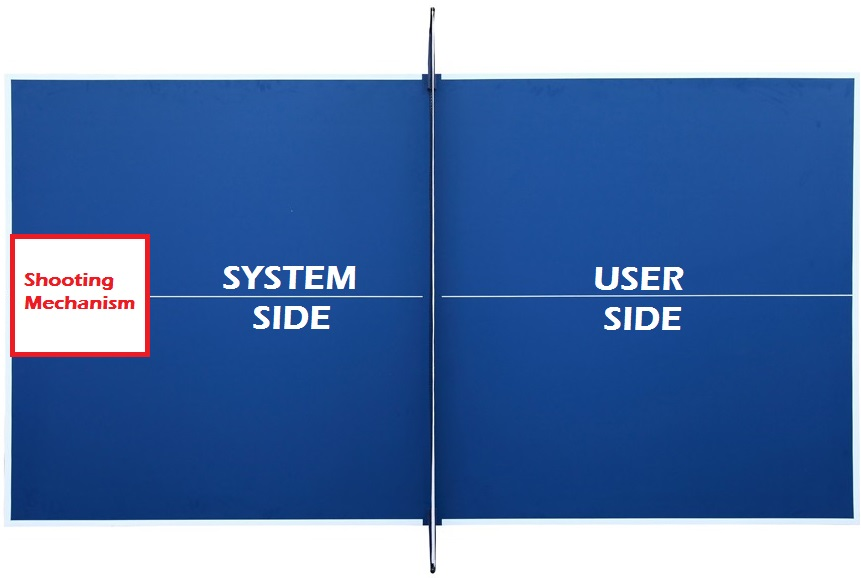
\includegraphics[width=1\textwidth]{../img/Table-Tennis-Top-View.png} % requires the graphicx package
   \caption{Top View of the Tennis Table}
   \label{fig:table-tennis-top-view}
\end{figure}
\subsection{Relevant Facts and Assumptions}
According to the International Table Tennis Federation (ITTF), the regulation table size is as follows: 2.74m long, 1.525m wide and 0.76m high off the ground. The table must be a uniformly dark in colour with a 2cm-thick white line along the edge of the table, as well one running parallel to the 2.74m side in the middle of the table. The net in the middle of the table must be 15.25cm vertically high from the table. A 3D representation of the table setup is illustrate in Figure \ref{fig:table-tennis-dim}.
\begin{figure}[htbp]
   \centering
   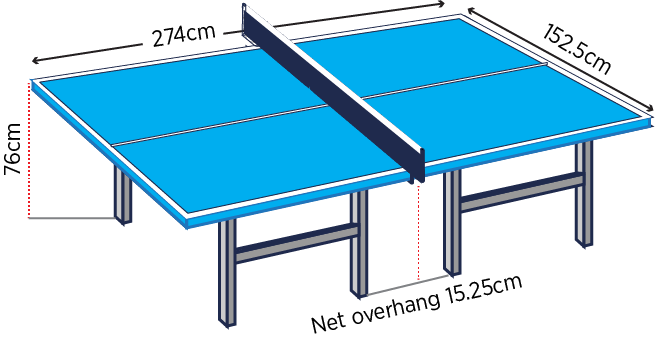
\includegraphics[width=0.7\textwidth]{../img/table-tennis-dim.png} % requires the graphicx package
   \caption{3D Tennis Table with Dimensions}
   \label{fig:table-tennis-dim}
   % The Laws of Table Tennis. ITTF Handbook 2016. www.ittf.com/ittf_handbook/ittf_hb.html
\end{figure} \\
During a singles gameplay, a valid serve must hit the server's side first, and then bounce once on the other player's side before being returned. After that is done, a valid return would be when the ball is hit by a player, after bouncing exactly once on their side, and bounces at least one time on the opposing player's side. If a serve touches the net and lands on the opposing player's side, it is a \textit{let}. No points are allocated and the turn must be re-served.
% TODO add user chars?
\section{Functional Requirements}

\subsection{The Scope of the Work and the Product}

\subsubsection{The Context of the Work}
% no idea what this means tbh
\subsubsection{Work Partitioning}
% what works gets done where, really to do with third parties
\subsubsection{Individual Product Use Cases}

\subsection{Functional Requirements}

\begin{framed}
	\noindent\textbf{Requirement \#}: -5 \hfill \textbf{Requirement Type}: F \hfill\\\\
	\noindent\textbf{Description}: This is an example, TODO remove!  \\
	\textbf{Rationale}: Why does this req exist, why is it REQUIRED? \\
	\textbf{Fit Criterion}: When is it satisfied? \\\\
	\textbf{Originator}: Christopher McDonald \\\\
	\textbf{Priority}: High/Med/Low \hfill \\
	\noindent\textbf{History}: Created 13-OCT-2017
\end{framed}


\section{Non-Functional Requirements}

\subsection{Look and Feel Requirements}

\subsection{Usability and Humanity Requirements}

\subsection{Performance Requirements}

\subsection{Operational and Environmental Requirements}

\subsection{Maintainability and Support Requirements}

\subsection{Security Requirements}

\subsection{Cultural Requirements}

\subsection{Legal Requirements}

\subsection{Health and Safety Requirements}

\section{Project Issues}

\subsection{Open Issues}
% things we know we will have a hard time doing, or not addressing
\subsection{Off-the-Shelf Solutions}
% actually refers to above issues
%Sharon: Is this more something that exists already?
\subsection{New Problems}
% maybe these are ones w/o solutions?
\subsection{Tasks}

\subsection{Migration to the New Product}

\subsection{Risks}

\subsection{Costs}

\subsection{User Documentation and Training}

\section{Anticipated Changes}

\section{Appendix}
% diagrams, tables, ... etc.

\subsection{Symbolic Parameters}
% The definition of the requirements will likely call for SYMBOLIC\_CONSTANTS.

\end{document}  